\documentclass[sigconf]{acmart}
% Cleaning 
\pagestyle{fancy} % removes running headers
\settopmatter{printacmref=false} % Removes citation information below abstract
\renewcommand\footnotetextcopyrightpermission[1]{} % removes footnote with conference information in first column
\pagestyle{plain} % removes running headers
\fancyhead{}
\settopmatter{printacmref=false, printfolios=false}
% Copyright
\setcopyright{none}
% \setcopyright{acmcopyright}
% \setcopyright{acmlicensed}
% \setcopyright{rightsretained}
% \setcopyright{usgov}
% \setcopyright{usgovmixed}
% \setcopyright{cagov}
% \setcopyright{cagovmixed}
\settopmatter{printacmref=false} % Removes citation information below abstract
\acmDOI{}

\usepackage{CJKutf8}
\usepackage{booktabs} % For formal tables
\usepackage{url}
\usepackage{hyperref}
\usepackage{algorithm}
\usepackage[noend]{algpseudocode}
\algtext*{EndWhile}% Remove "end while" text
\algtext*{EndIf}% Remove "end if" text
%\usepackage{flexisym}

\setlength{\parskip}{0pt}
\setlength{\parsep}{0pt}
\setlength{\headsep}{0pt}
\setlength{\topskip}{0pt}
\setlength{\topmargin}{0pt}
\setlength{\topsep}{0pt}
\setlength{\partopsep}{0pt}
%\linespread{0.95}
\usepackage{mdwlist}
\usepackage{amsmath}

\begin{document}
\title{Machine Translating From English to Chinese for E-Commerce Product Categorization}\titlenote{\href{https://github.com/duongy18418/Multilingual-NLP/tree/main/Code}{https://github.com/duongy18418/Multilingual-NLP/tree/main/Code}}

\author{Kitty Duong}
\affiliation{
  \institution{University of Windsor}
  \city{Windsor}
  \country{Canada}
}
\email{duongy@uwindsor.ca}

\author{Miaomiao Zhang}
\affiliation{
  \institution{University of Windsor}
  \city{Windsor}
  \country{Canada}
}
\email{zhang3s2@uwindsor.ca}

\begin{abstract}
This study explores the application of a machine translation model, Meta AI's NLLB-200\cite{Meta_AI_Research_Topic}, for the translation of Amazon product categories from English to Chinese. Given the critical role of accurate category translation in enhancing user experience and facilitating seamless e-commerce navigation, this research aims to evaluate the efficacy and accuracy of the NLLB-200 model against the existing Chinese categories on Amazon. Through a systematic translation of the sample data from Amazon and a comparison process between experiment results and the existing results, the study assesses the accuracy of NLLB-200 translations, identifying both the model's strengths and its limitations in handling e-commerce terminology. The findings indicate that while NLLB-200 shows promise in accurately translating a wide range of product categories, discrepancies in certain translations highlight areas for further refinement.\cite{moslem_2023} This research contributes to the ongoing discussion on improving machine translation for e-commerce applications and offers insights into the potential of NLLB-200 to support multilingual e-commerce platforms. The outcomes not only underscore the importance of leveraging advanced AI for localization efforts but also pave the way for future enhancements in machine translation technologies.

\end{abstract}

\keywords{Multilingual NLP, machine translation, e-commerce product categories, e-commerce translation, translation accuracy, translation evaluation}
\maketitle


\section{Problem Definition}
The global nature of e-commerce demands accurate and efficient localization of platform content, including product categories, to cater to diverse linguistic audiences. This localization is pivotal for user experience, searchable, and navigation efficiency on multinational platforms like Amazon. Traditional machine translation tools often struggle with maintaining accuracy, especially for languages with significant syntactic and semantic differences, such as English and Chinese.\cite{brazill_masters_munday_2017} Introducing advanced machine translation models like NLLB-200 offers a potential solution to these challenges by promising high-quality translations across a wide range of languages, including those less represented in digital resources.

However, the effectiveness of NLLB-200 in the specific context of e-commerce, particularly for the accurate translation of product categories from English to Chinese, remains an open question. Given the critical role of these categories in user interaction and the unique challenges posed by specialized e-commerce terminology, there is a pressing need to evaluate the performance of NLLB-200. This involves assessing its translation accuracy compared to manually curated categories on Amazon's Chinese platform and identifying any systematic discrepancies that could impact user experience.\cite{chang_2022} Addressing this problem requires a detailed analysis of NLLB-200's translation outcomes and a comparison framework that considers both direct translation accuracy and the semantic integrity of category labels.

\section{Proposed Approach}\label{approach}
Our proposed machine translation evaluation method aims to fine-tune a pre-trained model and further train it for e-commerce product category translation from English to Chinese, then compare the accuracy of the results with the existing Chinese version on Amazon, as defined in the previous section. The approach works through two pipeline phases: the translation process and the comparison framework. In the following subsections, we describe the details of each step.

\subsection{Translation Process}
In our approach, the translation process for converting Amazon product categories from English to Chinese using the NLLB-200 model\cite{Meta} entails preparing a standardized list of categories, setting up access to the NLLB-200 model through its API or SDK, and configuring translation parameters. Categories are then translated in batches, with errors and limitations managed appropriately. The resulting translations undergo initial review before being compared to Amazon's official Chinese categories to assess accuracy. The data of the experiment results would be stored in a file named "result.csv".


\subsubsection{Data Preparation}
In this experiment, we used the data from "Amazon\_Ecommerce\_Data\_2020.csv"\cite{PromptCloud} as the dataset, which could provide a comprehensive list of Amazon product categories in English. Due to the size of the dataset, we selected around 90 pieces of data by random, which covers a wide range of product categories, so that we could test the translation capabilities of NLLB-200 across different terminologies and contexts. 


\begin{algorithm}[t]
\caption{Finetuning and comparing process}
\label{bicluster}
\begin{algorithmic}[1]

\Statex\textbf{Inputs:} 
\Statex\hspace{\algorithmicindent} dataset $\mathbb{D}$, Amazon Chinese categories $\mathbb{Z}$, sample data $\mathbb{S}$
\Statex\textbf{Initialization:}
\Statex\hspace{\algorithmicindent} import transformer and datasets
\Statex\hspace{\algorithmicindent} load NLLB-200 Model
\Statex\hspace{\algorithmicindent} size of sample data = 90
\Statex\hspace{\algorithmicindent} size of accurate data = 0
\Statex\hspace{\algorithmicindent} $S\subset{D}, S = [d_1,d_2,d_3.....d_i]$
\Statex\textbf{Output:} 90 sample data in Chinese saved in result.csv 
\Procedure{finetune and compare}{}

\If{$(D!=\varnothing)\land(S\subset{D})$}
\ForAll{$d_i\in S$}
\State $d'_i\leftarrow finetune(d_i)$
\State $d'_i\in S'$
\EndFor
\EndIf
\ForAll{$d'_i\in\mathbb{S'}$}
\State $res\leftarrow ndiff(d_i,d'_i)$
\If{$res==true$} 
\State $acc\leftarrow acc+1$
\Else
\State get\_close\_matches($d_i,d'_i$)
\EndIf
\EndFor
\EndProcedure
\end{algorithmic}
\end{algorithm}

\subsubsection{Fine-tune NLLB-200 Model}
We utilized the API provided by MetaAI to set up an environment with any necessary dependencies and authentication for accessing the NLLB-200 model. Besides, we followed the tutorial from Hugging Face to use PyTorch Trainer to finetune the pre-trained model\cite{Hugging_Face}. Based on the configuration settings to specify the source (English) and target (Chinese) languages, we organized the product categories into batches for efficient processing, and then we sent batches to NLLB-200 for translation processing.

\subsubsection{Post-Translation Processing}
As for the experiment results, we stored the translated categories after the translation processing, alongside their original English counterparts in a file named "result.csv" for further analysis. For the initial quality assurance, we collected the existing Chinese categories from the Amazon website and then conducted a preliminary review of the translation results to identify any glaring errors or inconsistencies that could indicate issues with the translation process.


\subsection{Comparison Framework}
In this experiment, the comparison work would focus on semantic equivalence and terminology appropriateness between the experiment results and the existing Amazon Chinese version. Furthermore, discrepancies are documented, and a statistical analysis is conducted to evaluate NLLB-200's overall performance, aiming to highlight the model's strengths and areas for improvement in e-commerce localization.

For each translated category, we attempt to find an exact or closely matching category within Amazon's existing Chinese version. As for evaluating the accuracy of translation results, we need to consider factors such as semantic equivalence, appropriateness of terminology, and consistency with Amazon's category naming conventions.

As for the 90 pieces of testing data in this experiment, we did a manual review for the initial assessment of translation accuracy. The experiment result shows around 80\% of accurate translation compared with the Chinese version on the Amazon website. There would be some inappropriate translations concerning semantic analysis.\cite{palmer_wu_1995} For instance, the translation of the 7th testing data in the result.csv ("Window Treatments") is "\begin{CJK*}{UTF8}{gbsn}窗口治疗\end{CJK*}", which translated the whole vocabulary into two vocabularies separately. "\begin{CJK*}{UTF8}{gbsn}窗口治疗\end{CJK*}" means "window" plus "treatments" in Chinese, which is coming with no actual meanings. "Window Treatments" should be translated into "\begin{CJK*}{UTF8}{gbsn}窗上用品\end{CJK*}" or something similar, which means a set of decorations for a window, often including curtains or blinds.\cite{window_treatment_definition_meaning_yourdictionary} Another example is the 9th testing data, the translation of "Baby\&Toddler toys". The translation result is "\begin{CJK*}{UTF8}{gbsn}宝宝\end{CJK*}" for both "Baby" and "Toddler". There is a distinct difference between these two vocabularies, as "Baby" means kids at the stage from zero to twelve months while "Toddler" means kids at the stage from one to three years.\cite{american_academy_of_pediatrics_2019} Furthermore, there would be duplication errors for some testing data, the result is repeating the same characters.\cite{koponen_2010} As we could find from the comparison outcome in the experiment of the 90 pieces of testing data, the NLLB-200 model is unable to make appropriate translations for some data. 

As for the further analysis for semantic equivalence, appropriateness of terminology, and consistency with Amazon's category naming conventions, we would continue the evaluation process in the next stage, to provide a more specific and detailed analysis, which is expected to be implemented in Python via methods provided by Python API, such as "ndiff" method for detailed comparison and "get\_close\_matches" method for finding similar lines, \cite{difflib_helpers_for_computing-deltas_python_documentation}in which way we can acquire the completely same and similar results of all the pieces of data in the Amazon English categories.

\begin{figure}[t]
    \centering
    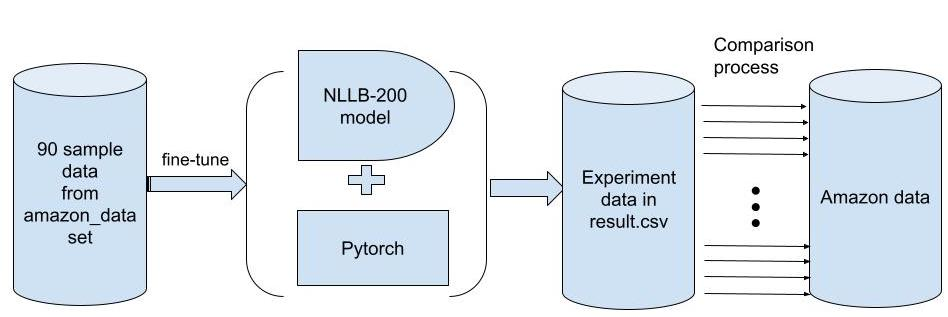
\includegraphics[width=1.1\linewidth]{illustrate_figure.jpeg}
    \caption{Finetune process architecture.}
    
\end{figure}

\bibliography{Bibliography.bib}
\bibliographystyle{acmart}

\end{document}


